\section{The token budget reshapes per-step cost}
\label{sec:budget}

vLLM caps the tokens one engine step may process with \texttt{max\_num\_batched\_tokens},
the token budget $B$. Its default on this GPU is 2048, which equalled the prompt
length in the experiments above. If the jump in per-step time comes from steps that
carry prompt chunks, the budget should control it.

\paragraph{Median against tail.}
At C32 we set the budget to 512, 2048, and 8192 (Table~\ref{tab:budget}). No setting wins on every metric:
\begin{itemize}
  \item \emph{512:} spreads prompt work into many small steps. ITL is nearly flat
    (p50 15.8\ms, p99 17.8\ms), but TTFT triples and throughput falls 10\%. Queueing
    takes two thirds of each request's latency (1.2 of 1.8\,s).
  \item \emph{2048 (the default):} most steps carry a full 2048-token chunk, so p50
    and p99 are both near 55--59\ms.
  \item \emph{8192:} batches several prompts into fewer, much larger steps. The
    median falls to 6.9\ms{} and throughput rises 18\%, but p99 rises to 169\ms.
\end{itemize}
The budget with the best median has the worst tail. By mean time per output token
after the first, $(\mathrm{E2E}-\mathrm{TTFT})/31$, the order is 512 (15\ms), 8192
(26\ms), and 2048 (45\ms). These descriptions of how each budget cuts prompt work into
steps were Phase D's post hoc reading; Milestone 5's step log later showed the step
sizes directly: at 2048, 77\% of steps carried prompt work, with a median of 2048
prompt-carrying tokens (Section~\ref{sec:stepcost}).
% src: reports/milestone3-20261006T022744Z-phase-d.md (Result table: queue 1222.3 of E2E 1843.9 ms at 512; mean E2E and TTFT per budget; prediction 7; prediction 10); reports/milestone5-*-pilot.md (step-log table, anchor-before)

\begin{table}[t]
  \centering
  \caption{Token budget at C32, prefill-heavy workload (2048/32 tokens). Medians of
    three repetitions.}
  \label{tab:budget}
  \begin{tabular}{rrrrr}
    \toprule
    Budget & ITL p50 (ms) & ITL p99 (ms) & Mean TTFT (ms) & Output tok/s \\
    \midrule
    512  & 15.8 & 17.8  & 1378.8 & 496.2 \\
    2048 & 55.4 & 58.6  & 432.7  & 550.8 \\
    8192 & 6.9  & 168.7 & 686.1  & 652.5 \\
    \bottomrule
  \end{tabular}
  % src: reports/milestone3-20261006T022744Z-phase-d.md (Part 2 table; predictions 7, 8, 10; Phase C bullet: 652.5 tok/s at 8192)
\end{table}


We had predicted that both ITL p50 and p99 would order 512 $<$ 2048 $<$ 8192. The
p99 ordering held and the p50 ordering did not. The manipulation check relied on
vLLM's iteration-token histogram, which cannot show per-step chunk sizes
(Section~\ref{sec:method}), and it failed as specified. Under the pre-registered rule,
that made the test of the mechanism inconclusive. If we accept server-log evidence
that the budgets were applied, which is a deviation from the protocol, the
pre-registered form of the step-size explanation, a p50 that rises with the budget, is
unsupported. The measured trade-off stands, and the open mechanism
motivated Milestone 5.
% src: reports/milestone3-*-phase-d.md (Falsification; prediction 6 failed as specified; prediction 7)

\paragraph{Prompt length against budget.}
Milestone 5 varied the prompt length $L \in \{1024, 2048, 4096\}$ at budgets 2048 and
8192 with the step log enabled (Table~\ref{tab:lengths}, Figure~\ref{fig:pilot}).
\begin{itemize}
  \item \emph{The budget sets the scale of the tail.} At $B{=}2048$, ITL p99 was
    58\ms{} for 2048-token prompts and 65\ms{} for 4096-token prompts. Past the budget,
    prompts are split into budget-sized chunks, so the tail grew only 11\%. At
    $B{=}8192$ the tail was about 3$\times$ higher (170 and 200\ms), while the median
    stayed below 10\ms.
  \item \emph{Prompts shorter than the budget did not shrink the tail as predicted.}
    The pre-registered prediction was that 1024-token prompts would have a tail at
    least 25\% lower than 2048-token prompts. It was 19\% lower. The step log suggests why
    (a post hoc reading): the scheduler packed two 1024-token prompts into one
    2048-token step (Section~\ref{sec:stepcost}).
  \item \emph{Concurrency moves the median.} At C8 with $B{=}2048$, ITL p50 was
    4.6--5.7\ms{} for every prompt length, against 55--57\ms{} at C32 for $L \ge 2048$
    (6.1\ms{} at $L{=}1024$, where prompts are packed), as predicted; only a minority
    of C8 steps carry prompt work. The tail fell less, to 40--54\ms. 1024-token prompts
    were packed at C8 as well (an 11\% lower tail, against a predicted 25\%). At C8
    with $B{=}8192$, prompt length did move the tail: p99 rose from 60 to 178\ms{}
    between $L{=}1024$ and $L{=}4096$.
\end{itemize}
% src: reports/milestone5-20261025T004640Z-pilot.md (Measurements; predictions 3-5); reports/milestone5p2-20261029T000043Z-part2.md (C8 table; predictions 8, 9)

\begin{table}[t]
  \centering
  \caption{Prompt length $L$ against budget $B$ at C32 and C8 (32 output tokens).
    ITL p50 / p99 in ms; medians of three repetitions.}
  \label{tab:lengths}
  \begin{tabular}{rrrr}
    \toprule
    $B$ & $L$ & C32 & C8 \\
    \midrule
    2048 & 1024 & 6.1 / 47.4  & 4.6 / 40.4 \\
    2048 & 2048 & 55.3 / 58.3 & 4.9 / 45.5 \\
    2048 & 4096 & 57.4 / 64.7 & 5.7 / 53.8 \\
    8192 & 1024 & 5.7 / 151.3 & 4.6 / 60.4 \\
    8192 & 2048 & 7.0 / 169.5 & 4.9 / 120.3 \\
    8192 & 4096 & 9.7 / 199.9 & 5.5 / 177.5 \\
    \bottomrule
  \end{tabular}
  % src: reports/milestone5-20261025T004640Z-pilot.md (Measurements, C32; L2048/B2048 is anchor-before); reports/milestone5p2-20261029T000043Z-part2.md (Part 2A table, C8)
\end{table}

\begin{figure}[t]
  \centering
  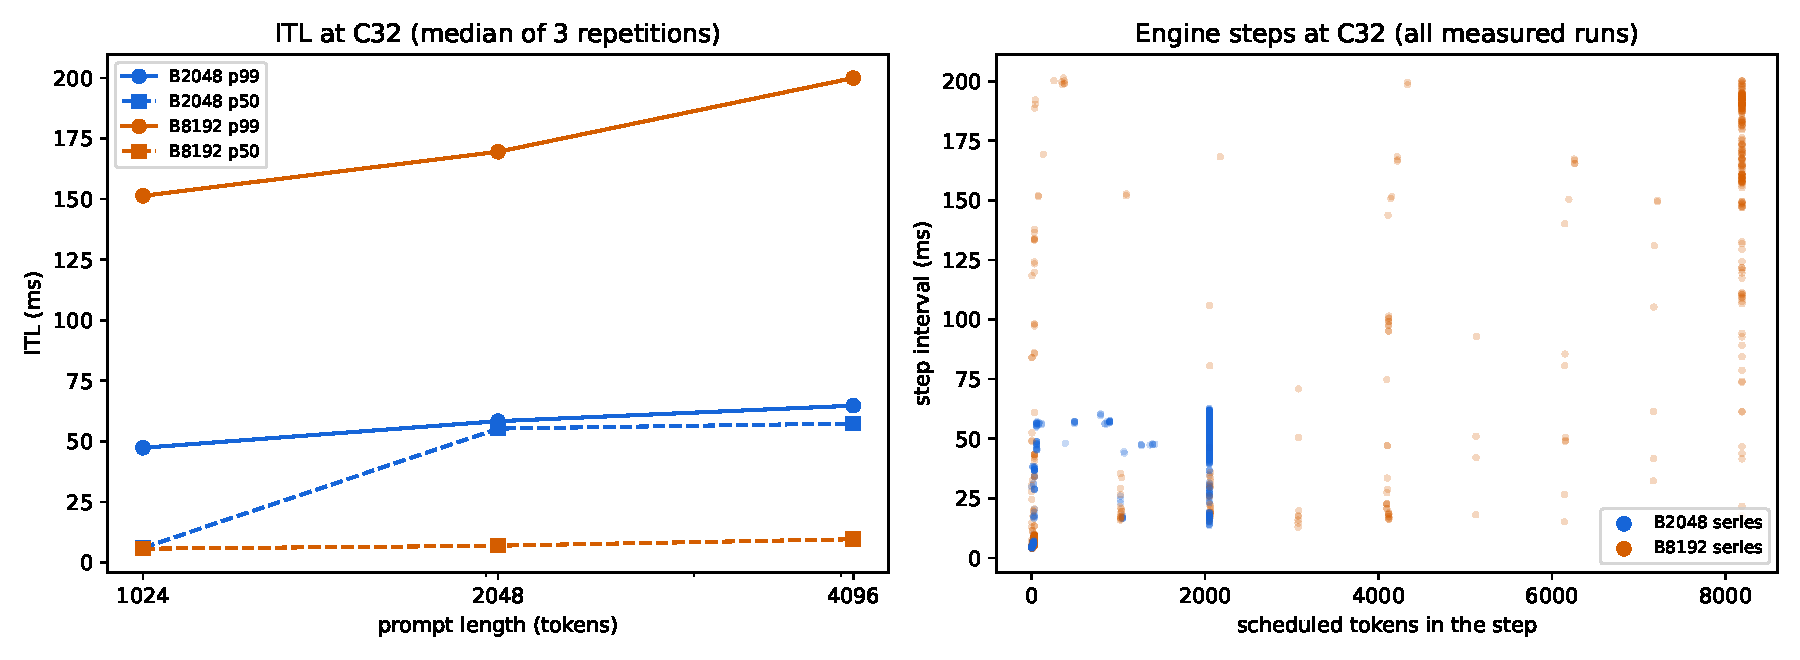
\includegraphics[width=\linewidth]{milestone5-pilot.pdf}
  \caption{Milestone 5 at C32. Left: ITL p50 and p99 by prompt length for each
    budget. Right: every measured engine step's interval (to the next step's start)
    against its scheduled tokens. This interval is confounded with the previous step
    (Section~\ref{sec:stepcost}).}
  \label{fig:pilot}
\end{figure}
